\documentclass{article}
\usepackage{graphicx}
\usepackage{amsmath}

\title{GATE Question}
\author{Anushree M R \ ID:COMETFWC063}
\date{}

\begin{document}

\maketitle

\section*{Question:41}

For any set of inputs $A$ and $B$, the following circuits give the same output $Q$ except one.
Which one is it? 

\section*{Options}

\begin{figure}[h]
\centering
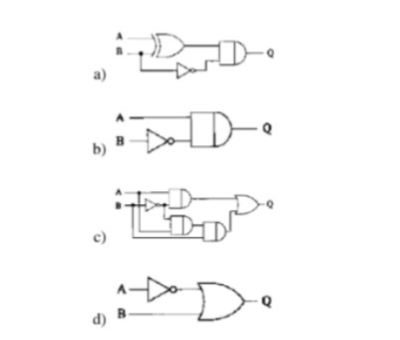
\includegraphics[width=0.6\textwidth]{figs/options.jpg}
\end{figure}

\section*{Solution}

By analysing the logic circuits:

\[
(a)\; Q = (A \oplus B)B^{'} = AB^{'}
\]

\[
(b)\; Q = AB^{'}
\]

\[
(c)\; Q = A
\]

\[
(d)\; Q = A^{'} + B
\]

Thus circuits (a) and (b) produce the same output $AB^{'}$.

Circuit (c) produces output $A$, which is different.

Therefore the circuit that gives a different output is

\[
\boxed{(c)}
\]

\section*{Graphical Verification}

\begin{figure}[h]
\centering
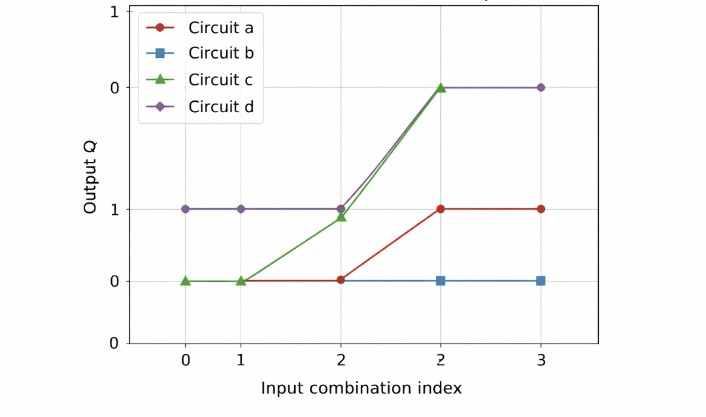
\includegraphics[width=0.7\textwidth]{figs/graph.jpg}
\end{figure}

\end{document}

